\documentclass{article}
%\usepackage{arxiv}

\usepackage{draftwatermark}
\SetWatermarkText{Draft Version}
\SetWatermarkScale{3}
\SetWatermarkColor[gray]{0.9}

\usepackage[utf8]{inputenc} % allow utf-8 input

\usepackage[T1]{fontenc}    % use 8-bit T1 fonts
\usepackage{url}            % simple URL typesetting
\usepackage{booktabs}       % professional-quality tables
\usepackage{amsfonts}       % blackboard math symbols
\usepackage{nicefrac}       % compact symbols for 1/2, etc.
\usepackage{microtype}      % microtypography
\usepackage{lipsum}
\usepackage{graphicx}
\usepackage{amsmath}
\usepackage{hyperref}       % hyperlinks

\title{Exploring Risks of Human Challenge Trials for COVID-19}


\author{Manheim, David$^{*+}$ \and Więcek, Witold$^*$ 
\and Virginia Schmit %\and Chris Choe \and Troy Yamaguchi \and Linchuan Zhang 
\\ \and Sophie Rose  \and Josh Morrison \and 1DaySooner Research Team}
\date{October 2020}

\begin{document}
\maketitle

\begin{abstract}
   Human Challenge Trials (HCTs) are a potential method to accelerate development of vaccines and therapeutics against COVID-19. However, HCTs may pose ethical and practical challenges due to the unclear and developing risks of COVID-19 infection. In this paper, we introduce an interactive model for exploring some risks of a SARS-COV-2 dosing study, a  prerequisite for any COVID-19 challenge trials. The risk estimates we use are based on a Bayesian evidence synthesis model which can incorporate new data on infection fatality rates (IFRs) to patients, and infer rates of hospitalization. We have also created a web tool to explore risk under different study design parameters and participant scenarios. Finally, we use our model to  from individual risk to the overall mortality and hospitalization risk in a dosing study.
   
   Based on the Bayesian model we expect IFR for someone between 20 and 30 years of age to be 17.3 in 100,000, with 95\% uncertainty interval from 12.8 to 23.6.  Using this estimate, we find that a simple 50-person dosing trial using younger individuals has a 99.1\% (95\% CI: 98.8\% to 99.4\%) probability of no fatalities, and a 92.8\% (95\% CI: 90.3\% to 94.6\%) probability of no cases requiring hospitalization. However, in a properly conducted HCT, the IFR will depend on the types of reductions may be achieved by a trial designer through screening for comorbidities and providing medical care, and we project this risk to be as low as 3.1 per 100,000, with a 99.85\% (95\% CI: 99.7\% to 99.9\%) chance of no fatalities, and a 98.7\% (95\% CI:  97.4\% to 99.3\%) probability of no cases requiring hospitalization.
\end{abstract}

\small{\noindent
*) Equal Contribution\\
+) Corresponding Author: david@1DaySooner.org}

\pagebreak

\section{Introduction}

As of November 1, 2020, severe acute respiratory syndrome coronavirus 2 (SARS-CoV-2) has led to almost 48 million confirmed infections worldwide and over 1.2 million deaths. Currently, there are no clinically-approved vaccines against COVID-19. McKinsey estimates that global vaccine capacity will reach one billion by the end of 2020 and eight billion by 2021 assuming all vaccine candidates pass clinical trials on time\cite{McKinsey2020}--a thin margin of error.

Timely development of new pharmacological therapeutics and vaccines will be necessary to manage disease burden and impact of COVID-19.
Unfortunately, traditional clinical trials are slow and require large subject populations to discern therapeutic effects. In order to accelerate testing, several authors and institutions have proposed intentionally exposing human subjects to SARS-CoV-2 to test novel interventions; to this date, nearly forty thousands of people have expressed interest in volunteering for this task\cite{1DSWeb}. Such human challenge trials (HCTs) have been useful in the past to develop vaccines and treatments for other infectious diseases such as Malaria, cholera, respiratory syncytial virus (RSV) \cite{roestenberg2018experimental, gomez2015controlled}, influenza \cite{treanor1999evaluation}, and Dengue fever \cite{larsen2015dengue}. However, two major problems currently stand in the way of conducting HCTs for SARS-CoV-2 infection. First, given lack of rescue therapies and our limited understanding of COVID-19’s risks, it is difficult to weigh the costs of these studies or give informed consent to volunteers\cite{palmer2020}. Second, we do not know what viral dose of SARS-CoV-2 should be given to volunteers. 

To help address both concerns, we developed a model to help assess the risks participants will face in a hypothetical dosing study for COVID-19. This model uses data from a non-systematic review of data on COVID-19 risks (mortality and infection rates) and describes risks for individuals as well as the overall study risk. As both clarification on viral dose and viral risk are essential before starting HCTs, this work can help inform policymakers and potential volunteers about some risks concerning the process of using HCTs to accelerate vaccine and therapeutic development.

\section{Methodology}

We developed a three-component tool to understand and explain the relevant risks. The first component quantifies risk of COVID-19 mortality by using a Bayesian evidence synthesis model; the second uses that estimate, along with other data on gender-specific mortality and hospitalization risks to simulate the risk of a study with given characteristics; the third is a front end tool for allowing interactive exploration of risks from a study or to an individual.

\subsection{Bayesian evidence synthesis model}

We use a Bayesian meta-analysis approach to obtain an estimate of mortality risk. This form of modelling combines different sources of evidence with varying statistical power to obtain posterior distribution for mortality risk in different populations. In our case, we use age-specific, location-specific death and prevalence data to generate an estimate of the infection fatality rate (IFR), and estimates of relative risk in healthy individuals (vs the general population) to understand risk reduction in individuals who would participate in an HCT. 

We use Bayesian methods because they allow us to best account for heterogeneity in IFRs across different populations (age groups, different countries and regions). Characterising this heterogeneity is important when assessing possible reductions in IFRs. For example, it can be argued that an HCT designer can use screening and provide medical care to achieve a rate of IFRs which is at least as low as the region or country with the lowest IFRs in our data\footnote{This is an assumption, and we allow users of the tool to choose to use the overall estimate across studies, or the expected lower risk.}.

Although existing statistical packages for meta-analysis (both Bayesian and frequentist) could easily be used to model event rates such as IFR\cite{wiecek_baggr_2020, carpenter_hierarchical_2016}, these models may not work when no deaths are observed, as is often the case for COVID-19 in younger populations. To address this, we use death data and estimates of prevalence as inputs instead of IFRs. We then construct a new, reproducible model for IFRs.

Methodological details of the model are described in the Appendix.
\footnote{\noindent Briefly, let $k$ index populations and $\text{loc}_k$ their locations (countries, regions). Let $d_k$ be observed deaths for data point $k$;  $\mu^{(p)}_k$ the reported mean prevalence and $\sigma^{(p)}_k$ its standard error, on logit scale; $n_k$ the total population; $X$ is a vector of median ages, expressed in decades and centered at 25 years. The hierarchical model is as follows:

\begin{align}
d_k & \sim \text{Binomial}(n_k, p_kIFR_k) \\
\text{logit}(p_k) & \sim \mathcal{N}(\mu^{(p)}_k, (\sigma^{(p)}_k)^2) \\
\text{logit}(IFR_k) &= \theta_{\text{loc}_k} + X\beta, \\
\theta_j & \sim \mathcal{N}(\tau, \sigma^2), \bigskip \text{where } j=1,\ldots,K_{loc}.
\end{align}

\noindent The parameters of the model are $p_k$, the true prevalence; $\theta$, location-specific (random) effects on IFR; $\beta$, (fixed) effect of age; $\tau$ and $\sigma$, the hyper-mean and hyper-scale parameters for IFR. We implement our model in Stan\cite{carpenter2017stan}, with weakly informative priors on all parameters. The prior for $\tau$ is centered at 1 death per 10,000 cases.}
We assume that the fixed effect of age and random effects of location on IFR are on logit scale, as is typical for meta-analysis models of binary data. 

However, while our IFR estimates capture average risks within different age groups and even heterogeneity across regions or countries, they still refer to the general population (of a given age, in a given location). A prospective HCT participant would be screened for health issues and comorbidities, further reducing the risk in comparison to the members of general population. To account for this, we perform an additional analysis using OpenSAFELY\cite{williamson_factors_2020}, a large observational dataset on COVID-19 mortality factors that includes comorbidity and age information, as well as data on gender, comparing the risk in general population to lower-risk subpopulation\footnote{The lower-risk group is defined as non-obese, non-smoking, and without the following risk factors (same as used by \cite{williamson_factors_2020}): asthma, other chronic respiratory disease, chronic heart disease, diabetes mellitus, chronic liver disease, chronic neurological diseases, common autoimmune diseases (Rheumatoid Arthritis (RA), Systemic Lupus Erythematosus (SLE) or psoriasis), solid organ transplant, asplenia, other immunosuppressive conditions, cancer, evidence of reduced kidney function, and raised blood pressure or a diagnosis of hypertension.}. Similarly to adjustment for heterogeneity across general populations, the adjustment for screening can be turned on or off in our tool.

Input data for the Bayesian IFR model is based on a non-systematic review of the literature and earlier meta-analyses, particularly by Levin \textit{et al} \cite{levin2020assessing}, but we have also opportunistically included other studies %\cite{hallal2020remarkable}
, and data from other official sources
%\cite{ItalyEpi2020}
, as is detailed in the appendix. However, the list of studies is not fixed, since new and better characterized datasets are becoming available over time. For this reason, we have made sure that incorporating additional prevalence and death data from newer studies and/or updated data sets is straightforward. We will continually update the model to assure that any estimates provided to participants or used for decisions include all relevant data, rather than only using data that was available when the analysis was first performed.

Based on the imputed IFR, we use the age- and gender-specific data from Salje et al. \cite{Salje208} on the rate of death of hospitalized patients to impute the relative risk of hospitalization based on our meta-analysis for mortality risk.

Our model is available publicly (together with input data and source code for the tool), under an open license, at \url{https://github.com/1DaySooner/RiskModel}.

\subsection{Transforming individual risk into study risk}

Once a suitable challenge virus is manufactured, itself a complex process \cite{catchpole2018manufacturing}, the risk of the individual from a challenge trial may still depend on the dose of virus given. The uncertainties about dose-response lead to a number of additional uncertainties about overall study risk. For other viruses, such as H1N1 and H3N2 influenza, a dose-response relationship has been found\cite{memoli2015validation, han2019dose}. The specific dose-response relationship, and its functional form must be determined experimentally, which is an outcome rather than an input of a dosing study like the one we are considering. This uncertainty is a key issue, so, as suggested by Morgan and Henrion\cite{morgan1990uncertainty}, we advise that this structural uncertainty should not be treated as a probabilistic variable, and instead sensitivity analysis should be used to enable the consideration of a range of plausible outcomes.

Given the specifics of a study design, the relationship between individual risk and the risks in the overall study is straightforward, assuming independence of risk between individuals in the study\footnote{The assumed independence is conditional on the age and health status of participants, and for dose-response studies, also infection severity by dose.}. The risk to an individual of severe disease in the study given dose $d$ is indicated $S_d$, and the risk of mortality is correspondingly $M_d$m so the probability that someone in a group of size $N$ experiences the corresponding outcome is $1-(1-S_d)^N$ and $1-(1-M_d)^N$. By simulating the probability of impact for each dosed group and, in the case of more complex studies, conditioning the trial of later groups on the results of earlier ones, we can find the overall risk in more complex studies.

Despite the ability to consider more complex study structures, we have restricted the main study design to a simple $N$-person study, which provides an upper bound\footnote{ This is equivalent to assuming that the risk of infection at each dose is above the threshold for infection to replace a dose-response curve.} However, the underlying model structure allows dose-dependent and/or conditional study designs, as necessary, to accommodate dose response information and allow for the simulation of more complex trials.

% \subsubsection{Optional - Dose Escalation Trial} Dose-response is often modelled by using a  sigmoidal relationship, where the probability of infection ranges from zero to certain, depending on the dose. \\ As we illustrate with a simple dose response curve, the study simulation allows for more complex trials. In a dose-escalation study, a low does is used on a small group, and response is measured. If insufficient response is observed, another group is administered a higher dose, and the dose is increased in stages with additional sets of volunteers until a sufficient response is observed. We therefore consider a 3-level dosing study with 10 participants at each potential dosing level, and a final 20 person validation cohort at the dosing level which first finds adequate response. \\ We therefore assume that the risk for below-sufficient doses is negligible, for the penultimate dose is near the median population risk, and that the final dosing level is at the 95th percentile population risk level...

\subsection{Interface}

The web tool we built allows exploration of two related types of risk. The first allows individuals to explore their personal risk, for example, by gender and age, if they volunteer to participate in a study, while the second displays overall risk of a single round dosing study with a given number of participants. Assumptions on study design and the underlying risk can be adjusted to allow interactive exploration by policymakers and participants.

In considering personal risk, the tool uses pre-calculated outputs from the risk model to calculate and display predictions for hospitalization rate and death rate for individuals as a function of age and sex. 

Deaths are further translated into micromorts--the expected number of deaths per million events, a standard method of showing mortality risk\cite{howard1980making} often used for patient consent \cite{ahmad2015micromort}. Hospitalization and other impacts which cannot be transformed into micromorts, are presented as probabilities\footnote{See discussion below about incorporating other risks in the model as more data becomes available.}. 

The tool allows both the public and policymakers alike to explore how overall risks change depending on differences in study design. This also helps maintain transparency into clinical trial design concerns, thereby better informing potential challenge trial volunteers. We also note that for trial designers and ethicists, the relationship between risk of different impacts and compensation is critical.\cite{grimwade2020payment,palmer2020, Blumenthal-Barbymedethics-2020-106901}.

The importance of transparency and public engagement has been widely noted in the literature on challenge trials\cite{jamrozik2020covid}. For this reason, the tool is available for public use, and is already being used to inform people who have volunteered to be contacted to potentially participate in a challenge trial\cite{1DSWeb}.

\section{Results}

The analysis dataset for age-specific IFRs contains 114 data points from 23 studies, with each containing between 3 and 11 different age groups; all data are presented in Table 2 in Appendix and are included in the code repository accompanying this paper. A glance at available data also confirms the necessity of using a more complicated modelling approach: out of 114 age-specific estimates, only 24 contain individuals aged between 20 and 30. However, out of these 24, only 2 have median age that falls between 20 and 30.

The basic evidence synthesis model, which includes all of the data, but does not adjust for health status, finds that average IFR in 20-29 age group for the studies included in this analysis is 17.5 per 100,000 cases (95\% uncertainty interval\footnote{All intervals reported here are Bayesian posterior intervals. For brevity we just refer to them as "x\% interval".} 12.7 to 23.3). 
Extending the HCT population to also include 30-39 year olds would lead to mean IFR of 29.9 per 100,000 (95\% interval 21.9 to 39.9).

Based on OpenSAFELY data, we estimate that in healthy population (defined as lack of any co-morbidities listed above), the average mortality risk in
20-29 year olds is 1.9 times lower than in the general population, with 95\%  interval from 1.3 to 2.8.\footnote{Expanding to 20-39 year olds only slightly increases the risk reduction factor from 1.9 to 2.}

\begin{figure}
    \centering
    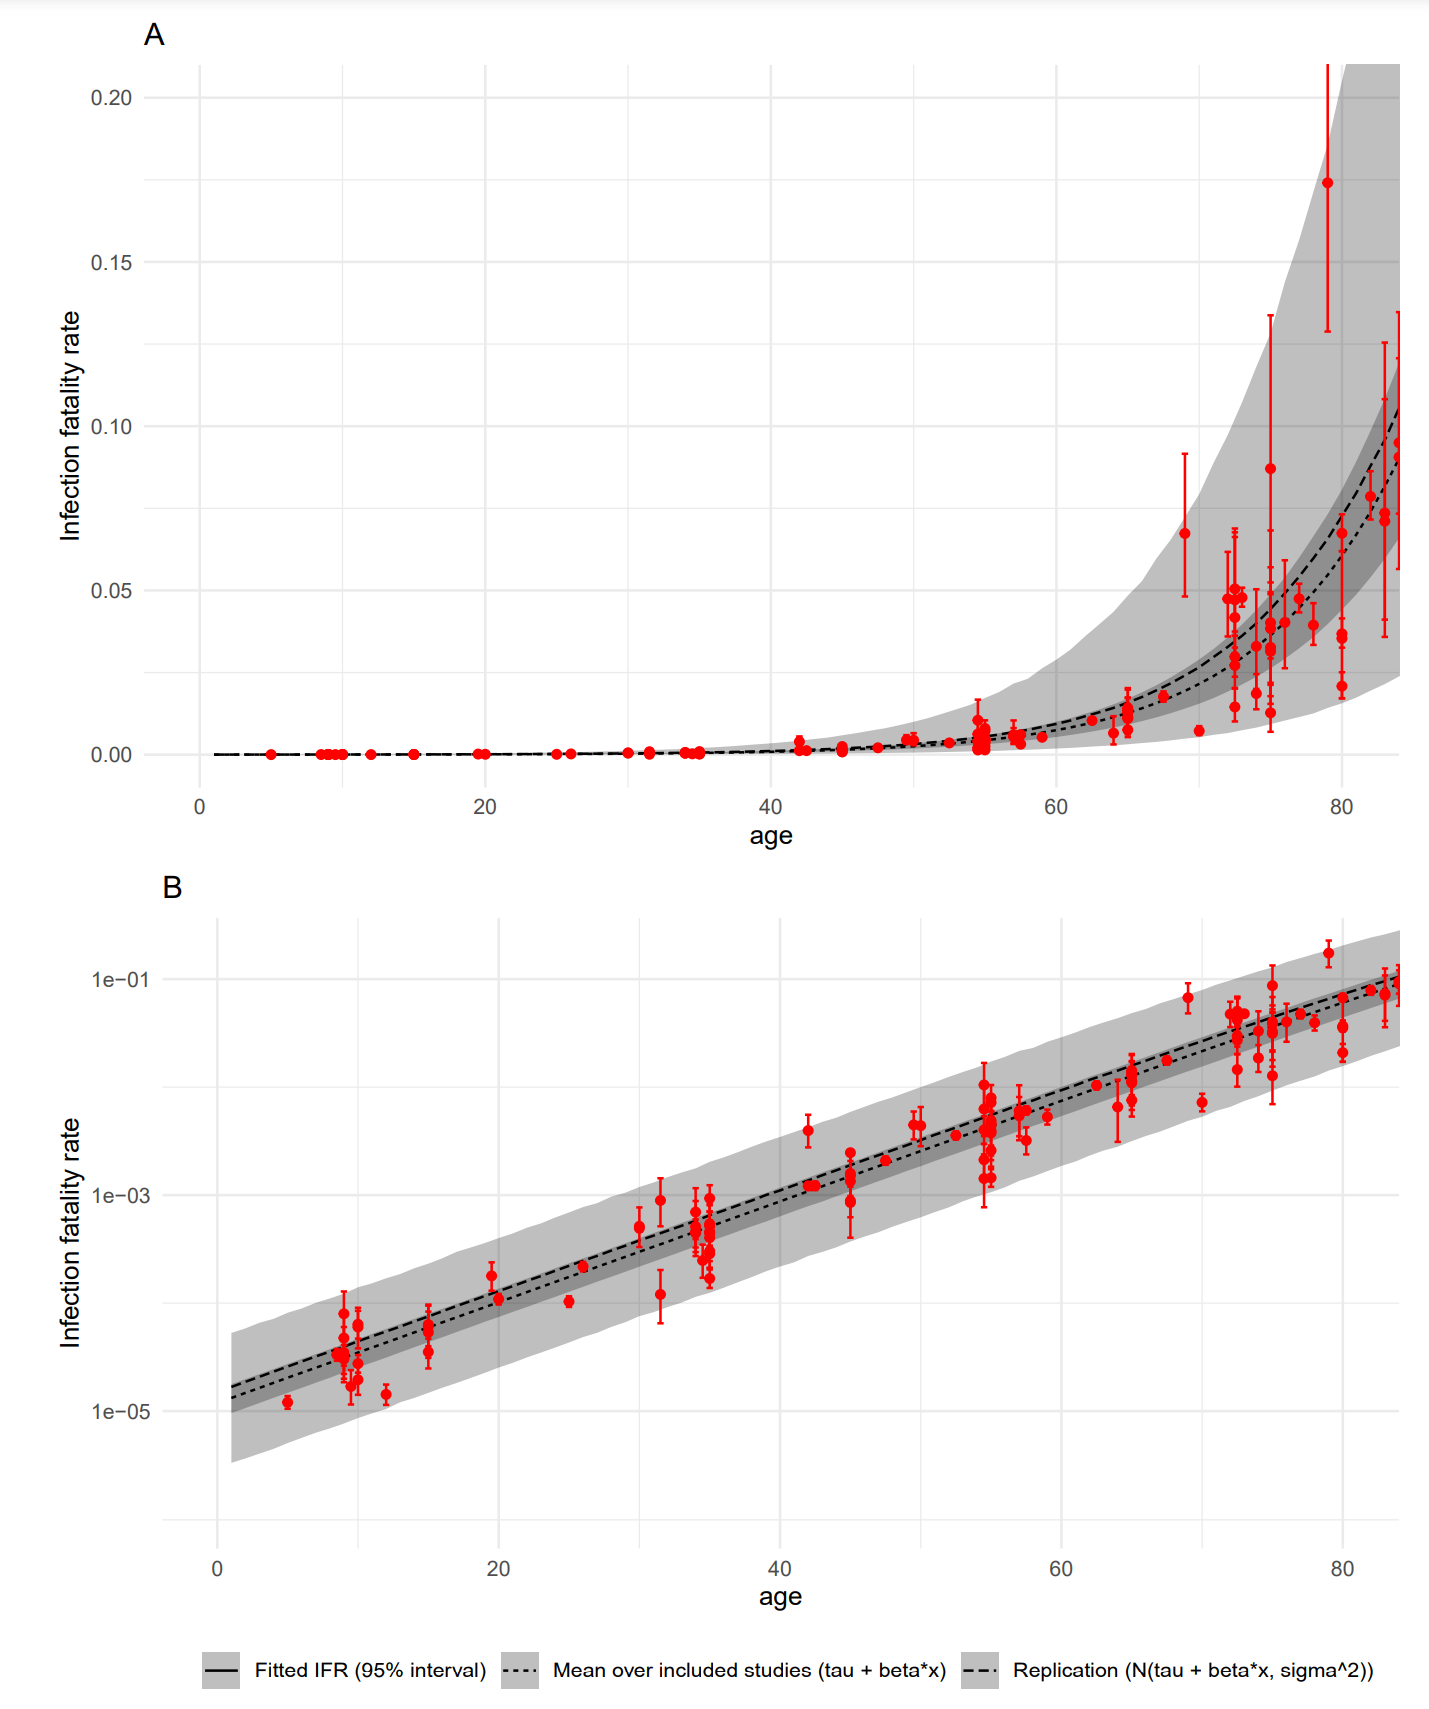
\includegraphics[width=12cm]{risk_estimate_fig1.png}
    \caption{IFR as a function of age. Panel A is untransformed data. Panel B shows the same data on log 10 scale. Red points are data, \textit{i.e.} model estimates of mean IFRs in particular studies, with bars representing 95\% posterior intervals. Black and gray are modelled IFRs: lines are means, ribbons are 95\% posteriors intervals: the narrower is average across all included studies, the wider takes into account heterogeneity between studies. Details and input values are given in Appendix.}
    \label{fig:my_label}
\textbf{Figures will be higher res in the final version.}
\end{figure}

We also note that there is large heterogeneity across the studies, due to treatment availability and other factors\footnote{Denoting by $\sigma$ the hyper-scale parameter in the hierarchical model, $2\sigma$ impact corresponds to 3.96-fold mean decrease in IFR. That means we expect 2.5\% of studies to have IFR more than 4 times lower than the average IFR.}. Because the HCT volunteer population will receive the best available care, including the most up-to-date treatment options, we can consider our population akin to a best-case scenario. In Belgium, the estimated risk for 20-29 year olds is $5.74 \times 10^{-5}$, approximately $\frac{1}{3}$ the estimated risk across all populations. Expanding the study population to 20-39 year olds would result in mean IFR of 9.88 per 100,000 cases.

Additionally, in the meta-analysis we estimate a population-level IFR by age, which does not account for the health status of screened volunteers. Looking at the OpenSAFELY dataset for the UK, we find a mean risk reduction factor in healthy populations aged 20-29 equal to 1.9, although our estimate is uncertain, with 95\% interval from 1.3 to 2.8. This adjustment can be used to modify the risk estimate for the general population across studies.

It is unclear how much double-counting occurs when adjusting for both available medical care and for screening out comorbidities. However, using this estimate, we use our estimate that a simple 50-person challenge trial has a  99.85\% probability of having no fatalities, and a 98.6\% probability of having no cases serious enough to require hospitalization.

The current model does not include estimates of longer term impacts due to lack of reliable data, but the model and interface can be updated with such estimates as they become available.

The model interface can be used to explore how these uncertain factors can interact, as shown below in Figure \ref{fig:webinterface}.
\begin{figure}
    \centering
    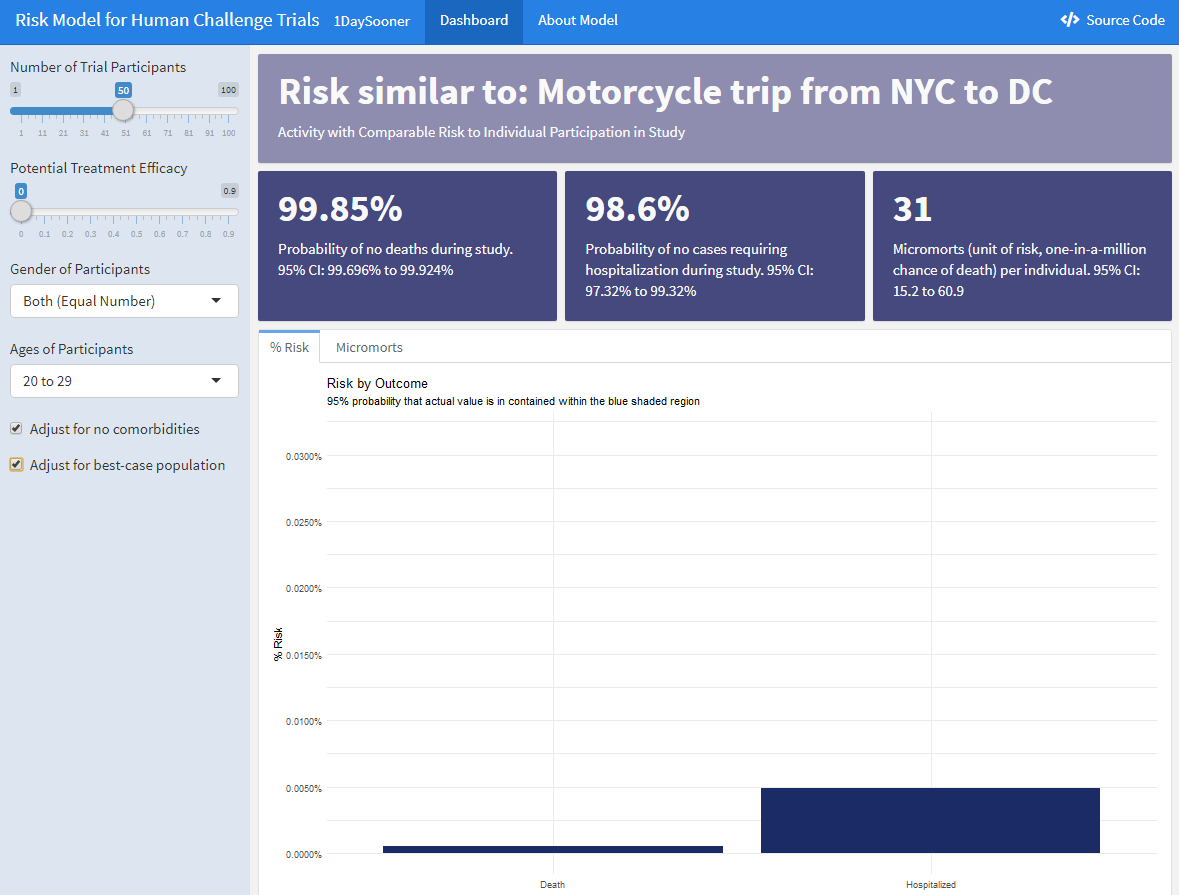
\includegraphics[scale=0.33]{RiskModelInterface.png}
    \caption{Interactive Model Interface}
    \label{fig:webinterface}
\end{figure}

The overall study risk for a simple 50 person study is 0.15\% probability of any deaths, and 1.4\% probability of at least 1 hospitalization. This represents an upper bound of risk for 3 groups 10 of volunteers given different doses of COVID-19, and an additional 20 person cohort to ensure sufficient sample size.

While the estimate is specific to a dosing study, it can also be useful for understanding the risk of later vaccine trials, though in that case other factors, including the possibility of vaccine-enhanced infection, would need to be assessed.

% \subsection{Optional - Dose Escalation} If a dose-escalation design is used, the previous estimate would not account for the probability of early stopping. This can be simulated in the model, given a distribution of uncertainty around the outcomes of each dose. The figure below shows the risk for various dose-response curves. (Probably a figure of color-coded graphs of different dose-response curves.)



\section{Discussion}

We have demonstrated that we can model certain risks associated with human challenge trials. However, our model is incomplete, and considerable concerns remain about the risks of human challenge trials. While a full accounting of challenge trial ethics is beyond the scope of this paper, we consider several factors below that inform our work on human challenge trial design, especially unmodeled risks. For a more complete perspective on the ethics of COVID-19 HCTs, we direct the reader to the World Health Organizations' (WHO) key considerations \cite{world2020key} and the recent discussion in Lancet Infectious Disease \cite{jamrozik2020covid,manheim2020evolving} on how these issues are being addressed. 

In our modal case, it is clear that the risk of our dosage-response study is not higher (and indeed likely far lower) than the risk from comparable clinical infections in the general population, and are far lower than other risks that are typically widely viewed as acceptable. Further, human challenge trials have had historical precedent, showing promise for both less lethal human coronaviruses, and for yellow fever\cite{shah2017ethical}. They also provided early indications regarding the possible efficacy of a leading malaria vaccine candidate\cite{nielsen2018rts}. The discussions about earlier trials shows that the ethical challenges of HCTs should not be seen as unique, but rather as lying along a natural continuum of clinical studies \cite{franklin2001ethical}. That said, the initial human challenge trials should be held to high ethical standards, both for individual risks and to preserve public trust in scientific and medical progress. That includes emphasis on fully informed consent of the participants, and as noted by the WHO, higher than typical ethical standards\cite{world2020key}. 



\subsection{Opportunity Cost}

When evaluating clinical trial design, it is not sufficient to evaluate whether the proposed model is good \textit{ex nihilo}. One must consider whether the alternatives are better. The key benefit of a dosing study is to allow further research with challenge trials, and alternative clinical trial models have major practical difficulties and far higher costs in a variety of ways. While this is not relevant for the initial set of vaccines that are close to approval, the challenge of large scale trials is magnified for later vaccines.

For example, “standard” phase 3 efficacy trials for an ongoing novel pandemic rely on high numbers of trial participants, and require this large sample for each vaccine or treatment that is trialled. Such trials are relatively expensive, and expose more trial participants to negative side effects of a given treatment, so that in many scenarios HCTs have been shown to be superior \cite{berry2020cost}. Standard trials are also difficult to pursue after an initial vaccine is available, and in the likely and hoped-for case that there will soon be at least one vaccine, finding willing participants for later and perhaps more effective vaccines, or ones with fewer side effects, is harder, and the burden of proof for benefit is far higher, or not achievable given plausible sample sizes, without an HCT.

\subsection{Limitations}

Finally, it is important to note that our model does have limitations. Hospitalization rates and death for 20-30 year olds are rare; our prior knowledge on fatalities for this group are more uncertain due to limited data. Information on long-term damage caused by COVID-19 is similarly incomplete, and though this is discussed further below, our model does not currently account for that risk. Also note that although our model uses hospitalization as a proxy for the upper bound of serious nonfatal COVID-19 cases, more data is required to see if this is an accurate assumption. 

Finally, our model may not accurately capture any changing nature of COVID-19 risk over time. It also does not estimate any indirect risks of the study. 
We stress that our model is not a be-all end-all for risk analysis, but is instead a tool for conceptualizing the overall risk of a study of this nature for its participants.

\subsection{Non-modeled Risks}

We also note that there are several impacts we do not model in the study, most notably the concern about so-called Long-COVID, which is a catch-all term referring to a combination of persistent symptoms, i.e. slow recovery, and new post-recovery symptoms\cite{carfi2020persistent}. It is understood that for some cases, especially severe ones, recovery from COVID-19 can take months. In others, there are longer-term symptoms differing from those experienced during the infection, perhaps similar to Post-SARS syndrome\cite{perrin2020into, moldofsky2011chronic}. At the same time, COVID-19 recovery has been found to be faster in younger, healthier patients\cite{tenforde2020symptom}, which may mean the risk is lower in this group. It seems clear that the risk is a subject of continuing scientific investigation, and as it becomes better understood and quantified, it will be incorporated into both the risk model, and the public interface.  

We also note that Vaccine-Enhanced disease is a critical concern for vaccine challenge trials, but is not relevant to dosing studies. Still, this risk must be considered in analyses of risks for later trials, and the model would need to be adapted or supplemented to consider this.

\section{Conclusion}
Human Challenge Trials are not risk free, but the balance of risk and benefits seems to clearly favor allowing them, as a large group of experts have argued. This conclusion is disputed by some, but all decisions are made despite uncertainties and debate - whether empirical or moral. \cite{lockhart2000moral, macaskill2020moral} The question is whether the both empirical and moral balance of factors lead to a viable conclusion. The alternative is analysis paralysis, or worse, using uncertainty and disputed moral claims as a positive stance to shut down further work, as has occurred in the debate about Human Challenge Trials\cite{martinez2020}.

It seems likely that Challenge Trials are a viable way to rapidly test vaccine efficacy, which is particularly critical now for testing second-generation vaccines, which may prove superior to first generation vaccines, or at least help fill the demand unmet by first-generation candidates. A dosing study is an urgent first step, and the risk estimates and tools developed for this paper can assist in planning such studies and informing volunteers. 

Our model provides insight into the overall risk of a trial of a given size, and can better inform HCT participants about the dangers they face. Given that an HCT may help select the multiple vaccines necessary for global immunization while also assisting with therapeutic testing, the risk tradeoff for this initial study into SARS-CoV-2 pathogenesis and developing model test vaccines seems worthwhile. Once the suggested dosing study is complete, an HCT for COVID-19 may provide a rapid and systematic way to screen vaccine candidates for efficacy and safety, which is a significant benefit.

The results presented are a useful static estimate of risk, but the framework and model used will allow for updating the model results with additional data as it becomes available. This contributes to the discussion of whether or not to pursue challenge trials, which can help with response to COVID-19 in a variety of ways\cite{Nguyen2020}. 

The model is already being used to inform potential volunteers \cite{1DSWeb}, and can be adapted and expanded to inform further work. Challenge trials may be an important tool for fighting COVID-19, and our model is a step towards that goal.\\


{\footnotesize{\textbf{Acknowledgements:} Thanks to Chris Choe, Troy Yamaguchi, and Linchuan Zhang for help preparing and editing the manuscript.}}

\bibliographystyle{plain}
\bibliography{references.bib}

\end{document}
